%%%%%%%%%%%%%%%%%%%%%%%%%%%%%%%%%%%%%%%%%%%%%%%%%%%%%%%%%%%%%%%%%%%%%%%%%%%
\section{\label{sec:Using-Condor-G}Using the Globus Universe}
%%%%%%%%%%%%%%%%%%%%%%%%%%%%%%%%%%%%%%%%%%%%%%%%%%%%%%%%%%%%%%%%%%%%%%%%%%%

\index{universe!Globus}
This section contains what users need to know to install Condor-G,
run, and manage jobs under
the globus universe.

%%%%%%%%%%%%%%%%%%%%%%%%%%%%%%%%%%%%%%%%%%%%%%%%%%%%%%%%%%%%%%%%%%%%%%%%%%%
\subsection{\label{sec:Grid-Access}Accessing the Grid with Condor-G}
%%%%%%%%%%%%%%%%%%%%%%%%%%%%%%%%%%%%%%%%%%%%%%%%%%%%%%%%%%%%%%%%%%%%%%%%%%%

Condor-G allows the user to treat the Grid as a local resource,
and the same command-line tools perform basic job management such as:
\begin{itemize}
\item Submit a job, indicating an executable, input and output files,
and arguments
\item Query a job's status
\item Cancel a job
\item Be informed when events happen,
such as normal job termination or errors
\item Obtain access to detailed logs that provide a complete history of a job
\end{itemize}

These are features that Condor has provided for many years.
Condor-G extends this to the grid,
providing resource management 
while still providing fault tolerance and exactly-once execution 
semantics. 

\begin{figure}[hbt]
\centering
\includegraphics{condor-g/gfig1.eps}
\caption{\label{fig:condorg}Remote Execution by Condor-G on Globus managed resources}
\end{figure}

Figure~\ref{fig:condorg} shows how Condor-G interacts with Globus protocols.
Condor-G contains a GASS server, used to transfer the executable,
\File{stdin}, \File{stdout}, and \File{stderr} to and from
the remote job execution site.
Condor-G uses the GRAM protocol to contact the remote Globus Gatekeeper
and request that a new job manager be started.
GRAM is also used to monitor the job's progress.
Condor-G detects and intelligently handles cases
such as if the remote Globus resource crashes.

%%%%%%%%%%%%%%%%%%%%%%%%%%%%%%%%%%%%%%%%%%%%%%%%%%%%%%%%%%%%%%%%%%%%%%%%%%%
\subsection{\label{sec:Condor-G-Install}Condor-G Installation}
%%%%%%%%%%%%%%%%%%%%%%%%%%%%%%%%%%%%%%%%%%%%%%%%%%%%%%%%%%%%%%%%%%%%%%%%%%%
\index{Condor-G!installation}
\index{contrib module!Condor-G}
\index{Condor-G!contrib module}
\index{installation!Condor-G contrib module}
There are two ways to obtain and install Condor-G.
The first and recommended method utilizes a full installation
of Condor together with a contrib module to acquire the
ability to submit globus universe jobs.
If a pool of machines running Condor \VersionNotice
already exists,
then the path to submitting globus universe jobs is quite short.

The second way to obtain Condor-G uses the GPT-packaged version.
GPT is the Grid Packaging Technology from NCSA,
the native packaging format for the Globus Toolkit(tm).
The GPT-packaged version of Condor-G will install
into an existing Globus Toolkit installation.
It is not capable of providing the functionality of a complete Condor pool,
but it does allow use of the Condor job queuing interface to the Grid.
It is appropriate for those who only want to submit jobs to
Globus-managed resources.

The following sections detail the installation and start up
of Condor-G based on these two ways.

%%%%%%%%%%%%%%%%%%%%%%%%%%%%%%%%%%%%%%%%%%%%%%%%%%%%%%%%%%%%%%%%%%%%%%%%%%%
\subsubsection{\label{sec:Condor-G-FullInstall}Full Install with Condor-G Contrib Module}
%%%%%%%%%%%%%%%%%%%%%%%%%%%%%%%%%%%%%%%%%%%%%%%%%%%%%%%%%%%%%%%%%%%%%%%%%%%
\index{Condor-G!installation with Contrib module}
Once Condor is obtained via download, installed, and configured,
(see manual
section~\ref{sec:install} on page~\pageref{sec:install})
there are three steps necessary before a globus universe job
can be submitted:

\begin{enumerate}

\item{Obtain the Condor-G contrib module.}
From the Condor home page,
\URL{http://www.cs.wisc.edu/condor/},
find and click on the Condor-G page.
Find and click on the Condor-G contrib module link.
After agreeing to the license,
find and click on the Condor-G module for the proper platform
to begin the transfer. 

After the transfer is complete, you will have received some text files
along with the file \File{condor-g.tar}.
Untar this file in the existing \MacroUNI{release} directory to 
produce the three files
\begin{verbatim}
    sbin/condor_gridmanager
    sbin/gahp_server
    etc/examples/condor_config.local.condor-g
\end{verbatim}

\item{Configure for Condor-G.}
To configure Condor to be able to run globus universe jobs,
import the contents of the file
\File{etc/examples/condor\_config.local.condor-g}
to the existing configuration file.

If Condor-G is installed as root, the file
set by the configuration variable
\Macro{GRIDMANAGER\_LOG} must have world-write permission.
The Gridmanager runs as the user who submitted the job,
so the Gridmanager may not be able to write to the ordinary 
\MacroUNI{log} directory.
The example configuration file sets the log file to be 
\begin{verbatim}
GRIDMANAGER_LOG = $(LOG)/GridLogs/GridmanagerLog.$(USERNAME) 
\end{verbatim}
Use of this definition of \MacroNI{GRIDMANAGER\_LOG}
will likely require the creation of
the directory \verb@$(LOG)/GridLogs@.
Permissions on this directory should be set
by running \Prog{chmod} using the value 1777. 

Another option is to use the commented out configuration, located
directly below within the example configuration file,
to set \MacroNI{GRIDMANAGER\_LOG} with
\begin{verbatim}
GRIDMANAGER_LOG  = /tmp/GridmanagerLog.$(USERNAME)
\end{verbatim}

\item{Run Condor.}
Directions for running the Condor daemons do not change when using
the Condor-G contrib module.
See section~\ref{sec:Run-Condor} on page~\pageref{sec:Run-Condor}
for details.
\end{enumerate}

%%%%%%%%%%%%%%%%%%%%%%%%%%%%%%%%%%%%%%%%%%%%%%%%%%%%%%%%%%%%%%%%%%%%%%%%%%%
\subsubsection{\label{sec:Condor-G-GPTNMI}GPT NMI release including Condor-G}
%%%%%%%%%%%%%%%%%%%%%%%%%%%%%%%%%%%%%%%%%%%%%%%%%%%%%%%%%%%%%%%%%%%%%%%%%%%
\index{Condor-G!installation with GPT NMI release}
\Todo

%%%%%%%%%%%%%%%%%%%%%%%%%%%%%%%%%%%%%%%%%%%%%%%%%%%%%%%%%%%%%%%%%%%%%%%%%%%
\subsection{\label{sec:Running-CondorG-Job}Running a Globus Universe Job}
%%%%%%%%%%%%%%%%%%%%%%%%%%%%%%%%%%%%%%%%%%%%%%%%%%%%%%%%%%%%%%%%%%%%%%%%%%%
\index{Condor-G!job submission}

Under Condor, successful job submission to the Globus universe requires
credentials.
An X.509 certificate is used to create a proxy,
and an account, authorization, or allocation to use a grid resource
is required.
For more information on proxies and certificates,
please consult the Alliance PKI pages at 

\URL{http://archive.ncsa.uiuc.edu/SCD/Alliance/GridSecurity/}

Before submitting a job to Condor under the Globus universe,
make sure you have your Grid 
credentials and have used \Prog{grid-proxy-init} to create a proxy.

A job is submitted for execution to Condor using the
\Condor{submit} command.
\index{Condor commands!condor\_submit}
\Condor{submit} takes as an argument
the name of a file called a submit description file.
\index{submit description file!globus universe}
The following sample submit description file runs a job on
the Origin2000 at NCSA.

\begin{verbatim}
executable = test
globusscheduler = modi4.ncsa.uiuc.edu/jobmanager
universe = globus
output = test.out
log = test.log
queue
\end{verbatim} 

The 
\AdAttr{executable}
for this example is
transferred from the local machine to the remote machine.
By default, Condor transfers the executable.
Note that this executable must be compiled for the correct
platform.

The \AdAttr{globusscheduler} command is dependent on the
scheduling software available on remote resource.
This required command will change based on the Grid resource
intended for execution of the job.

All Condor-G jobs (intended for execution on Globus-controlled
resources) are submitted to the globus universe.
The \verb@universe = globus@ command is required
in the submit description file.

No input file is specified for this example job.
Condor transfers the output file produced 
from the remote machine to the local machine during execution.
The log file is maintained on the local machine.

To submit this job to Condor-G for execution on the
remote machine, use
\begin{verbatim}
condor_submit test.submit
\end{verbatim}
where \File{test.submit} is the name of the submit description file.

Example output from 
\Condor{q} for this submission looks like:
\begin{verbatim}
% condor_q


-- Submitter: wireless48.cs.wisc.edu : <128.105.48.148:33012> : wireless48.cs.wi

 ID      OWNER         SUBMITTED     RUN_TIME ST PRI SIZE CMD
   7.0   epaulson     3/26 14:08   0+00:00:00 I  0   0.0  test

1 jobs; 1 idle, 0 running, 0 held
\end{verbatim}

After a short time, Globus accepts the job.
Again running \Condor{q} will now result in

\begin{verbatim}
% condor_q


-- Submitter: wireless48.cs.wisc.edu : <128.105.48.148:33012> : wireless48.cs.wi

 ID      OWNER         SUBMITTED     RUN_TIME ST PRI SIZE CMD
   7.0   epaulson     3/26 14:08   0+00:01:15 R  0   0.0  test

1 jobs; 0 idle, 1 running, 0 held
\end{verbatim}

Then, very shortly after that, the queue will be empty again,
because the job has finished:

\begin{verbatim}
% condor_q


-- Submitter: wireless48.cs.wisc.edu : <128.105.48.148:33012> : wireless48.cs.wi

 ID      OWNER            SUBMITTED     RUN_TIME ST PRI SIZE CMD

0 jobs; 0 idle, 0 running, 0 held
\end{verbatim}


A second example of a submit description file runs the Unix \Prog{ls}
program on a different Globus resource.

\begin{verbatim}
executable = /bin/ls
Transfer_Executable = false
globusscheduler = vulture.cs.wisc.edu/jobmanager
universe = globus
output = ls-test.out
log = ls-test.log
queue
\end{verbatim} 

In this example, the executable (the binary) is pre-staged.
The executable is on the remote machine, and it is not to
be transferred before execution.
Note that the required 
\AdAttr{globusscheduler} and \AdAttr{universe}
commands are present.
The command
\begin{verbatim}
Transfer_Executable = FALSE
\end{verbatim}
within the submit description file identifies the executable
as being pre-staged.
In this case, the 
\AdAttr{executable}
command gives the path to the executable on the remote machine.

A third example shows how
Condor-G can set environment variables for a job.
Save the following Perl script with the name \File{env-test.pl},
and run the Unix command
\begin{verbatim}
chmod 755 env-test.pl
\end{verbatim}
to make the Perl script executable.

\begin{verbatim}
#!/usr/bin/env perl

foreach $key (sort keys(%ENV))
{
   print "$key = $ENV{$key}\n"
}

exit 0;
\end{verbatim}

Now create the following submit file
(Replace \File{biron.cs.wisc.edu/jobmanager} with a resource
you are authorized to use.):

\begin{verbatim}
executable = env-test.pl
globusscheduler = biron.cs.wisc.edu/jobmanager
universe = globus
environment = foo=bar; zot=qux
output = env-test.out
log = env-test.log
queue
\end{verbatim}

When the job has completed, the output file \File{env-test.out}
should contain something like this:

\begin{verbatim}
GLOBUS_GRAM_JOB_CONTACT = https://biron.cs.wisc.edu:36213/30905/1020633947/
GLOBUS_GRAM_MYJOB_CONTACT = URLx-nexus://biron.cs.wisc.edu:36214
GLOBUS_LOCATION = /usr/local/globus
GLOBUS_REMOTE_IO_URL = /home/epaulson/.globus/.gass_cache/globus_gass_cache_1020633948
HOME = /home/epaulson
LANG = en_US
LOGNAME = epaulson
X509_USER_PROXY = /home/epaulson/.globus/.gass_cache/globus_gass_cache_1020633951
foo = bar
zot = qux
\end{verbatim}


Of particular interest is the GLOBUS\_REMOTE\_IO\_URL environment variable.
Condor-G automatically starts up a GASS remote I/O
server on the submitting machine.
Because of the potential for either side of the connection to fail,
the URL for the server cannot be passed directly to the job.
Instead, it is put into a file, and the GLOBUS\_REMOTE\_IO\_URL
environment variable points to this file. 
Remote jobs can read this file and use the URL it contains
to access the remote GASS server running inside Condor-G.
If the location
of the GASS server changes (for example, if Condor-G restarts),
Condor-G will contact the Globus gatekeeper and update this file on
the machine where the job is running.
It is therefore important that all accesses to
the remote GASS server check this file for the latest location.

The following Perl script will use the GASS server in Condor-G
to copy input files to the execute machine.
(In our case, our remote job
is just going to count the number of lines in a file.
Hopefully, your job will be a bit more productive.)

\begin{verbatim}
#!/usr/bin/env perl
use FileHandle;
use Cwd;

STDOUT->autoflush();
$gassUrl = `cat $ENV{GLOBUS_REMOTE_IO_URL}`;
chomp $gassUrl;

$ENV{LD_LIBRARY_PATH} = $ENV{GLOBUS_LOCATION}. "/lib";
$urlCopy = $ENV{GLOBUS_LOCATION}."/bin/globus-url-copy";

# globus-url-copy needs a full pathname
$pwd = getcwd();
print "$urlCopy $gassUrl/etc/hosts file://$pwd/temporary.hosts\n\n";
`$urlCopy $gassUrl/etc/hosts file://$pwd/temporary.hosts`;

open(file, "temporary.hosts");
while(<file>) {
print $_;
}

exit 0;
\end{verbatim}

Our submit file looks like this:

\begin{verbatim}
executable = gass-example.pl
globusscheduler = biron.cs.wisc.edu/jobmanager
universe = globus
output = gass.out
log = gass.log
queue
\end{verbatim}

There are two optional submit description file commands
of note:
\AdAttr{x509userproxy} and
\AdAttr{globusrsl}.
The \AdAttr{x509userproxy} command specifies the path to
an X.509 proxy.
The command is of the form:
\begin{verbatim}
x509userproxy = /path/on/file/system
\end{verbatim}
If this optional command is not present in the submit description file,
then Condor-G checks the value of the environment variable
\Env{X509\_USER\_PROXY} for the location of the proxy.
If this environment variable is not present, then Condor-G
looks for the proxy in the file
\File{/tmp/x509up\_u0000},
where the trailing zeros in this file name are
replaced with the Unix user id.

The \AdAttr{globusrsl} command is used to add additional
attribute settings to a job's RSL string.
The format of the \AdAttr{globusrsl} command is
\begin{verbatim}
globusrsl = (name=value)(name=value)
\end{verbatim}
An example of this command in a submit description file
\begin{verbatim}
globusrsl = (project=Test_Project)
\end{verbatim}
This example's attribute name for the additional RSL is
\verb@project@, and the value assigned is \verb@Test_Project@.

%%%%%%%%%%%%%%%%%%%%%%%%%%%%%%%%%%%%%%%%%%%%%%%%%%%%%%%
\subsection{\label{sec:Condor-G-Credentials}Configuration and Credential Management}
%%%%%%%%%%%%%%%%%%%%%%%%%%%%%%%%%%%%%%%%%%%%%%%%%%%%%%%

The following are required configuration file entries that
relate to submission of globus universe jobs.
Condor-G fails if any of these entries are missing.
These entries are provided in the file
\File{etc/examples/condor\_config.local.condor-g}
that is used during the installation of the Condor-G contrib module.

\begin{verbatim}
GRIDMANAGER             = $(SBIN)/condor_gridmanager
GRIDMANAGER_LOG         = $(LOG)/GridmanagerLog
MAX_GRIDMANAGER_LOG     = 64000
GRIDMANAGER_DEBUG       = D_COMMAND
GAHP                    = $(SBIN)/gahp_server
\end{verbatim} 

\AdAttr{GRIDMANAGER}
gives the path to the gridmanager daemon.
The 
\AdAttr{GRIDMANAGER\_LOG}
and
\AdAttr{MAX\_GRIDMANAGER\_LOG}
entries give the location of and how long
the log files may be.
\AdAttr{GRIDMANAGER\_DEBUG}
sets a debugging level for the gridmanager daemon.
The
\AdAttr{GAHP} entry specifies the location of the required
GAHP (Globus ASCII Helper Protocol) server.
Details of the protocol may be found at
\URL{http://www.cs.wisc.edu/condor/gahp/}.

Further configuration file entries are for the gridmanager daemon,
and they are relevant to
the newest job managers from the Globus 2.0 version of software.
\begin{verbatim}
GRIDMANAGER_CHECKPROXY_INTERVAL = 600
GRIDMANAGER_MINIMUM_PROXY_TIME = 180
\end{verbatim} 

Condor-G periodically checks for an updated proxy at
an interval given by the configuration variable
\AdAttr{GRIDMANAGER\_CHECKPROXY\_INTERVAL}.
The value is defined in terms of seconds.
For example, if you create a 12-hour proxy, and then
6 hours later re-run \Prog{grid-proxy-init},
Condor-G will check the proxy within
this time interval, and use the new proxy it finds there.
The default interval is 10 minutes.

Condor-G also knows when the proxy of each job will expire,
and if the proxy is not refreshed before
\AdAttr{GRIDMANAGER\_MINIMUM\_PROXY\_TIME}
seconds before the proxy expires,
Condor-G will shut down.
In other words, if
\AdAttr{GRIDMANAGER\_MINIMUM\_PROXY\_TIME}
is 180, and the proxy is 3 minutes away from
expiring, Condor-G will attempt to safely shut down,
instead of simply losing
contact with the remote job because it is unable to authenticate it.
The default setting is 3 minutes (180 seconds).

% other variables that should probably get documented
%GRIDMANAGER_CONTACT_SCHEDD_DELAY
%GRIDMANAGER_JOB_PROBE_DELAY
%GRIDMANAGER_RESOURCE_PRODBE_DELAY
%GRIDMANAGER_MAX_PENDING_SUBMITS
%GRIDMANAGER_GAHP_CALL_TIMEOUT
%GRIDMANAGER_SYNC_JOB_IO_INTERVAL
%GRIDMANAGER_MAX_PENDING_REQUESTS
%GAHP_ARGS
